\documentclass[10pt]{article}
\usepackage[margin=1.7cm]{geometry}
\usepackage{libertine}
\usepackage{amsmath, amssymb}
\usepackage{physics}
\usepackage{xcolor}
\usepackage{tikz}
\usetikzlibrary{quantikz}
\pagestyle{empty}
\setlength{\parindent}{0pt}
\setlength{\parskip}{0.5em}

\definecolor{accent}{HTML}{1E5C8A}
\definecolor{panel}{HTML}{EEF3F8}

\newcommand{\heading}[1]{{\bfseries\color{accent} #1}}

\begin{document}

{\LARGE\bfseries\color{accent} Quantum Computing Notes}\\[0.1em]
{\large Lecture 4: single-qubit gates, superposition, and measurement}

\vspace{0.7em}
\heading{1. The qubit}

A qubit's state is a normalized vector in a two-dimensional Hilbert space,
written in braket notation as
\[
  \ket{\psi} = \alpha \ket{0} + \beta \ket{1}, \qquad |\alpha|^2 + |\beta|^2 = 1,
\]
where $\ket{0}$ and $\ket{1}$ form the computational basis. The amplitudes
$\alpha,\beta \in \mathbb{C}$ are not directly observable; only the
probabilities $|\alpha|^2$ and $|\beta|^2$ of measuring $\ket{0}$ or $\ket{1}$
are. The inner product of two states $\braket{\phi}{\psi}$ gives their
overlap, and $\bra{\phi}\psi\rangle = \overline{\braket{\psi}{\phi}}$.

\heading{2. Single-qubit gates}

The Hadamard gate creates an equal superposition,
\[
  H\ket{0} = \frac{1}{\sqrt{2}}\big(\ket{0} + \ket{1}\big), \qquad
  H\ket{1} = \frac{1}{\sqrt{2}}\big(\ket{0} - \ket{1}\big),
\]
and the Pauli operators $X$, $Y$, $Z$ act as
\[
  X = \begin{pmatrix} 0 & 1 \\ 1 & 0 \end{pmatrix}, \quad
  Y = \begin{pmatrix} 0 & -i \\ i & 0 \end{pmatrix}, \quad
  Z = \begin{pmatrix} 1 & 0 \\ 0 & -1 \end{pmatrix}.
\]
A general single-qubit gate is any unitary $U$ with $U^\dagger U = I$; every
such $U$ can be written as a rotation about some axis of the Bloch sphere up
to a global phase.

\vspace{0.5em}
\noindent
\begin{minipage}[t]{0.52\textwidth}
\heading{3. A small circuit}

\vspace{0.4em}
The circuit below prepares a Bell pair from $\ket{00}$: a Hadamard on the
first qubit followed by a controlled-NOT entangles the two qubits into
$\frac{1}{\sqrt{2}}(\ket{00} + \ket{11})$.

\vspace{0.6em}
\begin{center}
\begin{quantikz}
\lstick{$\ket{0}$} & \gate{H} & \ctrl{1} & \qw \\
\lstick{$\ket{0}$} & \qw      & \targ{}  & \qw
\end{quantikz}
\end{center}

\vspace{0.5em}
{\small Reading left to right: time flows forward, each wire is one qubit,
and the filled dot with vertical line denotes the controlled-NOT.}
\end{minipage}%
\hfill
\begin{minipage}[t]{0.44\textwidth}
\heading{4. The Bloch sphere}

\vspace{0.4em}
\begin{center}
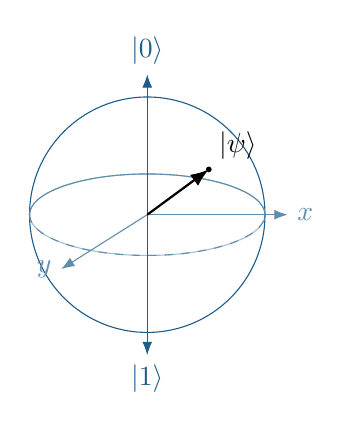
\begin{tikzpicture}[scale=1.15]
  \draw[accent!40] (0,0) ellipse (1.3 and 0.45);
  \draw[accent] (0,0) circle (1.3);
  \draw[accent!70, dashed] (-1.3,0) arc (180:360:1.3 and 0.45);
  \draw[accent!70] (-1.3,0) arc (180:0:1.3 and 0.45);
  \draw[-{Latex}, accent] (0,0) -- (0,1.55) node[above] {$\ket{0}$};
  \draw[-{Latex}, accent] (0,0) -- (0,-1.55) node[below] {$\ket{1}$};
  \draw[-{Latex}, accent!70] (0,0) -- (1.55,0) node[right] {$x$};
  \draw[-{Latex}, accent!70] (0,0) -- (-0.95,-0.6) node[left] {$y$};
  \draw[-{Latex}, black, thick] (0,0) -- (0.68,0.5) node[above right] {$\ket{\psi}$};
  \fill[black] (0.68,0.5) circle (0.9pt);
\end{tikzpicture}
\end{center}

\vspace{0.3em}
{\small Any pure state maps to a point on the unit sphere via
$\ket{\psi} = \cos\frac{\theta}{2}\ket{0} + e^{i\varphi}\sin\frac{\theta}{2}\ket{1}$.}
\end{minipage}

\heading{5. Measurement}

Measuring $\ket{\psi} = \alpha\ket{0} + \beta\ket{1}$ in the computational
basis yields outcome $0$ with probability $|\alpha|^2$, collapsing the state
to $\ket{0}$, and outcome $1$ with probability $|\beta|^2$, collapsing to
$\ket{1}$. For the Bell pair above, measuring the first qubit instantly
determines the second: the two outcomes are perfectly correlated even though
neither qubit alone carries that information.

\end{document}
